%==================== PARTE 3: RESULTADOS EXPERIMENTAIS (QUESTÃO 1) ====================
\section{Resultados experimentais da Questão 1: dados e método de análise}\label{expdados}
Nesta parte confronto os ensaios feitos na bancada (OpenPLC + Arduino + ScadaBR) com a simulação teórica das seções anteriores. Foram realizados quatro registros:
\begin{center}\small
\begin{tabular}{llp{8.2cm}}\toprule Arquivo & Item & O que foi feito\\\midrule
\texttt{Q11.csv} & 1.1 & Malha fechada com a sintonia de Dahlin; degrau de SP $19{,}5\to30\,\%$\\
\texttt{Q12.csv} & 1.2 & Transferência manual$\to$automático \emph{sem} VP-tracking (SP diferente da VP)\\
\texttt{Q13a.csv} & 1.3 & SP inalcançável (55\,\%) e retorno a 20\,\%, \emph{sem} anti reset windup\\
\texttt{Q13b.csv} & 1.3 & Mesma sequência, \emph{com} anti reset windup\\\bottomrule\end{tabular}\end{center}

\subsection{Formato dos arquivos e tratamento}
O ScadaBR grava um arquivo CSV em formato ``longo'': cada linha traz o \emph{nome do ponto} (\texttt{uno - SO}, \texttt{SP}, \texttt{VP}, \texttt{VP1}, \texttt{VP2}), o instante (data e hora, resolução de 1 s) e o valor. Os pontos são $SO=SC$ (sinal de controle), $SP$, $VP=\Vc3$, $VP1=\Vc2$ e $VP2=\Vc1$, todos em \% da escala (100\,\% $=5$ V). Como o número de linhas é diferente em cada variável (por exemplo, em \texttt{Q11.csv}: 2024 para SO e SP, 2028 para VP, 2020 para VP1, 2016 para VP2), \textbf{não se pode dividir o arquivo em 5 partes iguais} (como faz o script de exemplo do professor para arquivos com contagens idênticas). O código desta entrega separa as variáveis pelo \emph{nome}, coloca todas numa grade de 1 s e repete o último valor nos instantes sem registro (o código completo está no Apêndice~\ref{apcodigos}).
\begin{just}Os instantes são usados relativos a um evento (início da malha fechada, degrau de SP etc.). A diferença de horário entre o relatório em PDF do ScadaBR e o CSV é só de fuso/formatação e não afeta a análise.\end{just}

\subsection{Premissas}
\begin{enumerate}
\item \textbf{Sintonia usada nos quatro ensaios:} a de Dahlin do item 1.1 ($K_p=3{,}523$; $T_i=90{,}99$ s; $T_d=11{,}11$ s; $\mu=0{,}1$). Os números dos parâmetros digitados não estão nos arquivos; a evidência de que são esses vem do próprio dado: no degrau de SP da Q11, o SO saltou de $49{,}5$ para $86{,}5$\,\% (+$37{,}0$ pontos) para um degrau de SP de $10{,}48$ pontos, o que dá $K_p=37{,}0/10{,}48=3{,}53$, igual ao previsto $3{,}523$. \textbf{Confirme}, na sua anotação do ensaio, se os valores digitados foram esses.
\item \textbf{Limites do SC:} em todos os quatro arquivos o SO nunca saiu da faixa $[9{,}99;\,99{,}94]\,\%$ (o mínimo $9{,}99485$ e o máximo $99{,}940875=100\cdot1023/1024$ se repetem em todos). Ou seja, o sinal de controle está limitado, na prática, a \textbf{$\approx10\,\%$ (e não 0\,\%) até $\approx99{,}94\,\%$}. Nas simulações aplico esses mesmos limites.
\item \textbf{Modelo da planta:} FT completa das seções 2 e 3 (com os $R$ e $C$ medidos), mais um deslocamento (\emph{offset}) de saída obtido do ajuste da Seção~\ref{expplanta}.
\end{enumerate}
\subsection{O simulador de comparação}
Simulo a malha fechada em tempo discreto (passo 0,05 s) com a planta de 3ª ordem completa:
\[
x[k+1]=\Phi\,x[k]+\Gamma\,u[k],\quad \Phi=e^{A\,\Delta t},\ \Gamma=A^{-1}(\Phi-I)B,\qquad VP=x_3+\text{offset},
\]
com $A$ e $B$ da Seção 2 (espaço de estados da Lista 2). O controlador é o PI\_D do OpenPLC: $u=K_pe+I-D_{filtr}(VP)$, com $I[k+1]=I[k]+K_ie\,\Delta t$, derivada sobre a VP com filtro de constante $\mu T_d$, saturação em $[10;\,99{,}94]$ e anti-windup por \emph{clamping} (para de integrar quando $u$ está saturado e o erro empurra mais para a saturação). Na partida, o estado do circuito é o de regime correspondente ao $SO$ manual e a integral recebe o valor desse $SO$ (transferência sem solavanco, que é o que o bloco faz quando $SP=VP$).
\begin{formula}Métricas usadas: erro RMS e erro máximo entre VP experimental e VP simulada, $\varepsilon_{rms}=\sqrt{\frac1N\sum_k(VP_{sim,k}-VP_{exp,k})^2}$, $\varepsilon_{max}=\max_k|VP_{sim,k}-VP_{exp,k}|$ (em \% da escala). Para o SC uso a \emph{mediana móvel} do SO (explicado na Seção~\ref{expruido}).\end{formula}

%------------------------------------------------------------------
\section{Validação do modelo da planta com os dados do dia}\label{expplanta}
Antes de avaliar o controlador, confirmo que o modelo representa o circuito \emph{nos dias do experimento}.

\textbf{Ganho estático.} Nos patamares de regime em malha aberta (SO constante), obtive os pares:
\begin{center}\small
\begin{tabular}{ccc}\toprule SO [\%] & VP [\%] ($\Vc3$) & $VP/SO$\\\midrule
10,37 & 3,81 e 3,92 & 0,367 e 0,378\\ 20,00 & 7,70 & 0,385\\ 50,00 & 19,43 & 0,389\\ 99,94 & 39,39 & 0,394\\\bottomrule\end{tabular}\end{center}
A razão $VP/SO$ cresce com o SO, então não é um simples ganho proporcional: há um \emph{deslocamento}. A regressão linear dá
\[
VP=0{,}3963\,SO-0{,}262,
\]
isto é, \textbf{inclinação $0{,}3963$ (teórico: $K_3=0{,}3971$, diferença de 0,2\,\%)} e um offset de $-0{,}26$ ponto percentual. O offset é compatível com o ADC/saída do Arduino; a inclinação concorda com a teoria. Para os outros nós: com SO=99,94\,\% medi $VP1=58{,}85$ e $VP2=86{,}70$, que dão $K_2\approx0{,}589$ (teórico 0,591) e $K_1\approx0{,}868$ (teórico 0,869).
\begin{just}O $K=0{,}3918$ da identificação da 1ª parte veio de outro arquivo (outra data e montagem); a diferença para $0{,}3963$ (1,2\,\%) está dentro das tolerâncias de $R$ e $C$ e das condições do dia. Para as simulações desta parte uso a inclinação e o offset do próprio dia dos ensaios.\end{just}

\textbf{Dinâmica.} Para testar a dinâmica sem depender do controlador, excitei o modelo com o \textbf{SO medido} (o que realmente foi aplicado, amostrado a 1 s) e comparei a VP resultante com a VP medida:
\begin{center}\small
\begin{tabular}{lcc}\toprule Registro & RMS [\%] & erro máx.\ [\%]\\\midrule
Q11 (t=1160--2191) & 0,50 & 1,56\\ Q12 (t=20--1075) & 0,20 & 0,65\\ Q13a (t=20--2100) & 0,81 & 4,13\\ Q13b (t=20--825) & 0,50 & 0,97\\\bottomrule\end{tabular}\end{center}
No degrau manual $10{,}37\to50\,\%$ da Q11, o modelo reproduz VP, VP1 e VP2 com RMS de 0,28; 0,56 e 0,66\,\%. \textbf{O modelo físico está validado}: qualquer diferença entre simulação e experimento nas seções seguintes vem do controlador/implementação (ruído, limites, anti-windup), não da planta.

%------------------------------------------------------------------
\section{Item 1.1 experimental (Q11): Dahlin com $\tau_c=40$ s}
\subsection{O que foi feito (linha do tempo extraída do arquivo)}
\begin{enumerate}
\item Manual com $SO=65{,}9\to10{,}4\to50{,}0\,\%$ (a malha fica em aberto; o SP \emph{acompanha a VP} enquanto está em manual, isto é, o bloco tem VP-tracking). Com $SO=50\,\%$ a VP estabiliza em $19{,}4\,\%$.
\item Em $t=1606$ s a malha é fechada com $SP=19{,}5\approx VP$: o SO continua em $\approx50\,\%$ (mediana $49{,}6\,\%$), isto é, \textbf{a transferência é suave} (sem VP-tracking haveria um salto; ver Q12).
\item Em $t=1654$ s: degrau de SP $19{,}52\to30{,}0\,\%$ ($\Delta SP=10{,}48$).
\end{enumerate}
\subsection{Resposta imediata do SC: confirma $K_p$}
No instante do degrau, o SO foi de $49{,}5$ para $86{,}5\,\%$:
\[
\Delta SC_{0^+}=K_p\,\Delta SP=3{,}523\cdot10{,}48=36{,}9\ \text{pontos (previsto)}\qquad\text{medido: }86{,}5-49{,}5=37{,}0\ \text{pontos.}
\]
Esse salto vem só da ação proporcional: a derivada age sobre a VP (e não sobre o erro) e a integral ainda não acumulou. Nos 4 s seguintes o SO sobe $\approx0{,}34$ ponto/s ($86{,}5\to86{,}9\to87{,}3\to87{,}6\to87{,}9$), em boa concordância com a taxa integral $K_ie=0{,}03872\cdot10{,}4=0{,}40$ ponto/s, descontado o efeito da derivada (a VP está começando a subir). Assim, \textbf{os parâmetros $K_p$ e $K_i$ do controlador do experimento são os previstos}.

\subsection{Comparação VP e SC}
\begin{figure}[H]\centering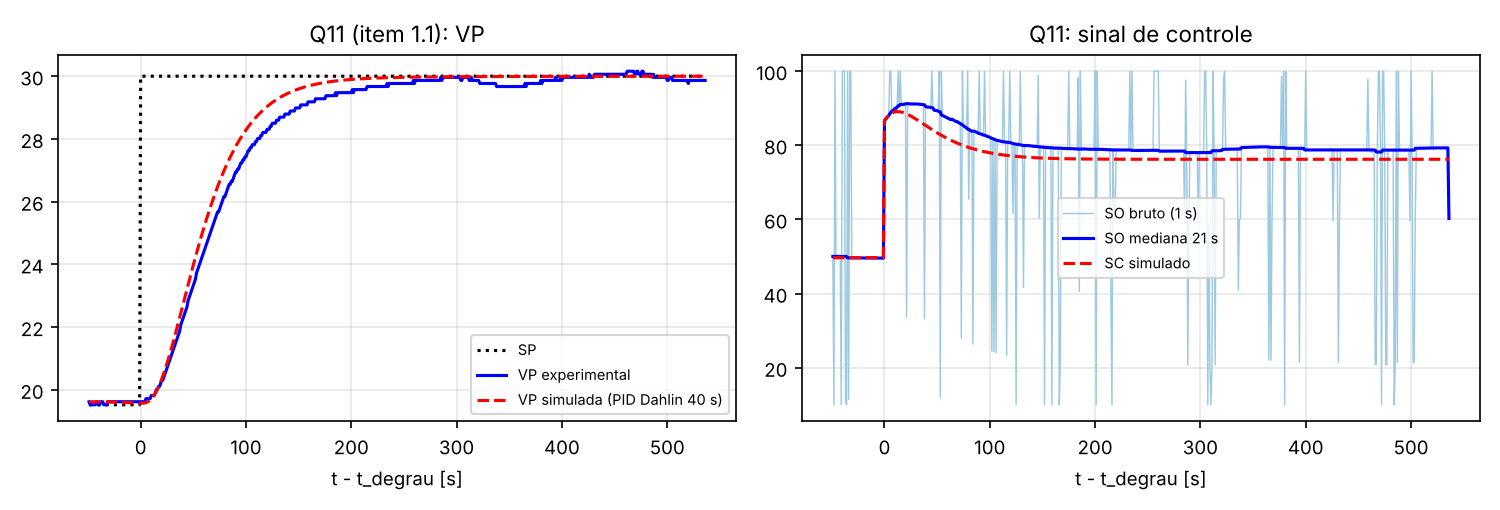
\includegraphics[width=.98\textwidth]{figs_exp/q11.png}\caption{Q11 (item 1.1). Esquerda: VP experimental (azul), SP e VP simulada. Direita: SO bruto (1 amostra/s, azul claro), mediana móvel de 21 s e SC simulado.}\end{figure}
\begin{center}\small
\begin{tabular}{lcc}\toprule & Experimento & Simulação (FT completa)\\\midrule
Instante em que a VP sobe 0,5 pt & 17 s & 16 s\\
$t_{28,3}$ / $t_{50}$ / $t_{63,2}$ & 43 / 64 / 79 s & 39 / 57 / 70 s\\
$t_{90}$ / $t_{95}$ / $t_{98}$ & 147 / 202 / 260 s & 118 / 142 / 174 s\\
Sobressinal (VP bruta) & 1,5\,\% ($VP_{max}=30{,}16$) & 0,0\,\%\\
SC médio em regime (últimos 300 s) & 75,4\,\% & 76,2\,\%\\
Erro VP: RMS / máximo & \multicolumn{2}{c}{0,38\,\% / 0,91\,\%}\\
Erro SC (mediana 21 s): RMS & \multicolumn{2}{c}{3,1\,\%}\\\bottomrule\end{tabular}\end{center}
\textbf{Interpretação.}
\begin{itemize}
\item \textbf{O sucesso da sintonia:} a VP chega ao SP sem sobressinal relevante ($\le1{,}5\,\%$ do degrau, no nível do ruído), com erro nulo em regime ($VP$ final $=29{,}9\text{--}30{,}0\,\%$), no formato previsto (sem oscilação, subida suave de 1ª ordem com atraso). O \emph{atraso aparente} de $\approx17$ s e o formato inicial são iguais aos simulados.
\item \textbf{A resposta experimental é um pouco mais lenta:} $t_{63,2}=79$ s contra 70 s (+13\,\%) e a cauda é mais lenta ($t_{98}=260$ s contra 174 s). As causas prováveis, em ordem: (i) as constantes de tempo reais do circuito são $\approx4$--6\,\% maiores que as calculadas (já constatado na identificação da 1ª parte, Seção 5.3); (ii) a rápida alternância do SO entre os limites (Seção~\ref{expruido}) \emph{retifica} o sinal: o SC médio aplicado ($75{,}4$) fica abaixo da mediana ($78{,}7$), o que atrasa o fechamento do último pedaço do degrau; (iii) tolerâncias dos $R$ e $C$.
\item \textbf{O SC concorda no valor médio e no formato:} salto inicial de $\approx37$ pontos, pico da mediana em $\approx91\,\%$ (simulado $88\,\%$) e queda até $\approx78$--79\,\% (simulado $76$). A diferença de $\sim3$ pontos entre mediana e simulação aparece porque o SO bruto é muito ruidoso; o que importa para a planta é a \emph{média}, e a média experimental ($75{,}4$) fica a $0{,}8$ ponto da simulada ($76{,}2$).
\end{itemize}
\begin{res}Item 1.1 verificado: a sintonia de Dahlin ($\tau_c=40$ s) leva a VP de $19{,}5$ a $30\,\%$ sem sobressinal significativo e sem erro em regime; VP experimental e simulada diferem por RMS de 0,38\,\% (3,6\,\% do degrau). O SC experimental tem o salto de $K_p\Delta SP$ previsto, mas é ruidoso (próxima seção).\end{res}

%------------------------------------------------------------------
\section{Por que o SO oscila entre $\approx$10\,\% e $\approx$99,9\,\% depois de fechar a malha? É preciso trocar para PI?}\label{expruido}
Esta é a observação mais importante dos ensaios: com a malha fechada, o gráfico do \texttt{SO} fica ``serrilhado'', com valores que pulam entre o limite inferior ($\approx10\,\%$) e o superior ($\approx99{,}9\,\%$), embora a VP seja suave. Vou mostrar, com os dados, \textbf{que isso não é instabilidade da malha}, qual é a causa, e o que fazer.

\subsection{Primeiro: não é instabilidade do laço}
\begin{itemize}
\item A \textbf{VP é suave}: em regime, o desvio-padrão da VP é de 0,13 ponto (Q11, $t>1900$ s), da ordem de 1 LSB do ADC ($0{,}0976\,\%$). Uma malha instável teria VP oscilando com amplitude crescente (como no ganho final do Z--N).
\item A \textbf{mediana} do SO é estável: desvio-padrão da mediana móvel $=1{,}2$ pontos (Q11), contra 17,5 do SO bruto.
\item O \textbf{valor médio} do SO está de acordo com a teoria: $(SP-\text{offset})/K=(30+0{,}26)/0{,}3971=76{,}2\,\%$ contra 75,4 medido.
\item Em Q11, 89,6\,\% das amostras do SO em malha fechada estão \emph{entre} os limites, só $2{,}4\,\%$ em 10\,\% e $8{,}0\,\%$ em 99,9\,\%: o SO fica no valor correto quase o tempo todo e dá \emph{picos isolados} ($\approx20\,\%$ das amostras).
\item Os picos já estão presentes com a \emph{malha recém-fechada e $SP=VP$} (Q11, t=1606--1650), quando o erro é praticamente zero e não há nada para ``instabilizar'' (veja a sequência do SO: \texttt{50, 50, 50, 10, 99,9, 50, 50, \ldots}).
\end{itemize}
\textbf{Conclusão parcial:} é um problema de \emph{ruído no sinal de controle}, e não de estabilidade.

\subsection{Segundo: a causa é a derivada atuando sobre a VP quantizada}
O ADC de 10 bits tem resolução de $100/1024=0{,}0976\,\%$ por degrau (LSB). A VP física varia lentamente (menos de $0{,}1\,\%$ por segundo em regime), então o valor lido é uma \textbf{escada}: fica constante por vários segundos e muda de 1 LSB de uma vez. Matematicamente, a derivada de uma escada é uma \emph{sequência de impulsos}. O termo derivativo é
\[
D(s)=\frac{K_d\,s}{\mu T_d\,s+1}\ \ \Rightarrow\ \ \text{resposta a um degrau de }\Delta V:\ \ u_D(t)=-\frac{K_d\,\Delta V}{\mu T_d}\,e^{-t/(\mu T_d)} .
\]
O sinal é negativo porque, no PI\_D, a derivada atua com sinal oposto sobre a VP. O \textbf{pico previsto por 1 LSB}, com o filtro funcionando como projetado ($\mu T_d=0{,}1\cdot11{,}11=1{,}11$ s), seria
\[
\frac{K_d\Delta V}{\mu T_d}=\frac{39{,}15\cdot0{,}0976}{1{,}11}=3{,}4\ \text{pontos},
\]
decaindo com constante de 1,11 s: um pequeno ``tremor'' de $\pm3$ pontos no SO. O ganho em alta frequência é $K_p(1+1/\mu)=38{,}8$: cada LSB vale $38{,}8\cdot0{,}0976=3{,}8$ pontos no máximo.

\textbf{O que os dados mostram é muito maior.} Nos registros com malha fechada:
\begin{center}\small
\resizebox{\textwidth}{!}{\begin{tabular}{lcccc}\toprule Registro & picos (|SO $-$ mediana|$>8$) & VP mudou 1 LSB & $P(\text{pico}\mid\text{LSB})$ & $P(\text{pico}\mid\text{sem LSB})$\\\midrule
Q11 ($t=1900$--2191) & 20\,\% das amostras & 14\,\% & 0,52 & 0,06\\
Q13a ($t=100$--560) & 46\,\% & 29\,\% & 0,64 & 0,27\\
Q12 ($t=620$--1075) & 42\,\% & 36\,\% & 0,56 & 0,22\\\bottomrule\end{tabular}}\end{center}
Na Q11 a probabilidade de haver um pico quando a VP muda de 1 LSB (na janela de $\pm1$ s) é $0{,}52$, \textbf{contra $0{,}06$ quando a VP não muda: um fator de 8,7}. Além disso, o \emph{sinal} é o da derivada sobre a VP: quando a VP sobe 1 LSB, o SO cai em média $26{,}1$ pontos; quando desce 1 LSB, o SO sobe em média $12{,}7$ (Figura~\ref{figruido}).
\begin{figure}[H]\centering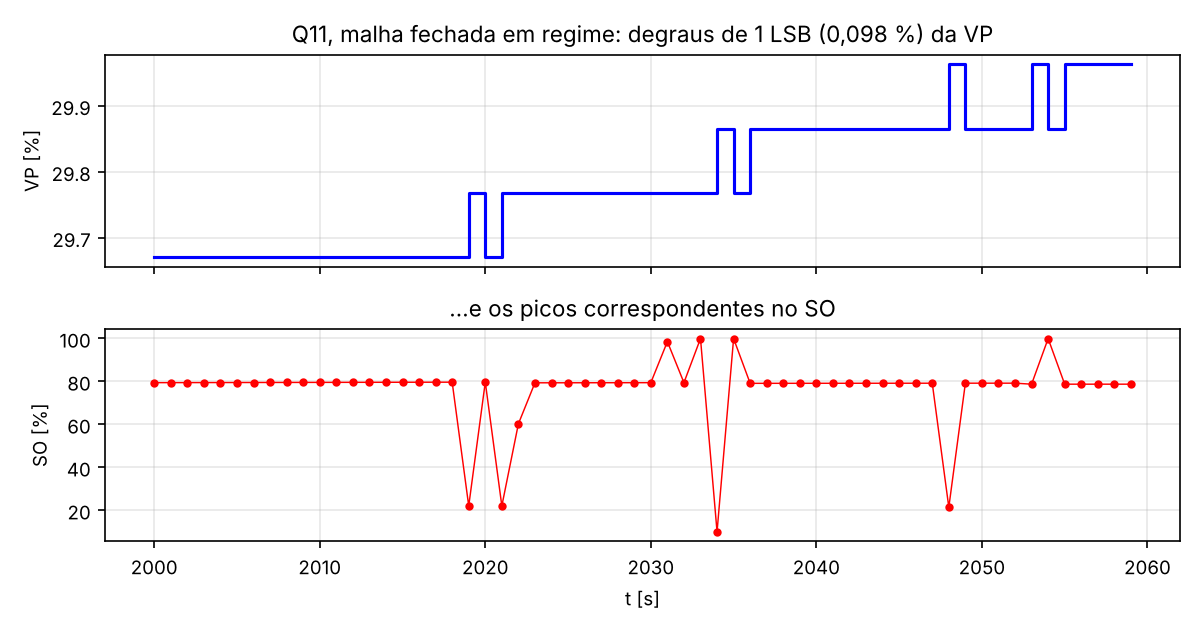
\includegraphics[width=.8\textwidth]{figs_exp/q11_ruido.png}\caption{Q11 em regime, malha fechada. Acima: a VP como escada de 1 LSB. Abaixo: o SO, com um pico a cada transição da VP.}\label{figruido}\end{figure}
\textbf{O tamanho do pico está inconsistente com o filtro de $\mu T_d=1{,}11$ s.} O pico típico medido (amostras não saturadas) tem mediana de 21 pontos, e muitos chegam a saturar (de $\sim79$ para 10 ou 99,9, isto é, $\gtrsim60$ pontos), contra os 3,4 pontos previstos. Como o ScadaBR só amostra o SO a cada 1 s (e um pico decai em fração de segundo), o pico real é ainda maior que o observado. Inverso: se o pico de 1 LSB é $K_d\Delta V/T_{ef}\gtrsim26$ pontos, então $T_{ef}\lesssim39{,}15\cdot0{,}0976/26=0{,}15$ s, muito menor que 1,11 s. Para comparação, uma derivada por \emph{diferença finita sem filtro}, com ciclo de execução (\emph{scan}) de 0,1 s, daria $K_d\Delta V/T_s=39{,}15\cdot0{,}0976/0{,}1=38$ pontos --- da ordem do observado.
\begin{alerta}Isto é uma \textbf{inferência}: não tenho o código do bloco PI\_D. O que os dados garantem é que (i) os picos acompanham as transições de 1 LSB da VP, com o sinal da derivada na VP, e (ii) são $\sim$10 vezes maiores do que o filtro $\mu=0{,}1$ permitiria. Isso indica que, no bloco usado, o filtro derivativo não está atuando como projetado (por exemplo, derivada calculada pela diferença entre amostras consecutivas do scan, com $\mu T_d$ muito curto na prática, ou $K_d$ digitado em unidade diferente da esperada). \textbf{Confirme:} (a) os valores de $K_d$, $T_d$ e $\mu$ digitados; (b) o tempo de ciclo do PLC; (c) o código do bloco.\end{alerta}

\subsection{Terceiro: por que o SO fica \emph{entre 10 e 99,9} e não entre $-\infty$ e $+\infty$}
Os picos de dezenas de pontos são cortados pelos limites do SC, $\approx10\,\%$ e $\approx99{,}94\,\%$ (Seção~\ref{expdados}). Por isso o gráfico parece ``instável entre 0 e 99'': na verdade é entre \textbf{10 e 99,94}, os limites de saturação. O limite inferior em 10\,\% (e não 0\,\%) aparece no mínimo $9{,}99485$ de todos os arquivos.

\subsection{Por que a planta ``não liga'' para os picos --- e por que ainda assim eles importam}
O circuito RC é um filtro passa-baixa de 3ª ordem (polos em $1/68{,}7$; $1/16$; $1/10{,}4$ s$^{-1}$): um pico de 60 pontos que dura $\sim0{,}2$ s muda a VP em centésimos de ponto. Por isso a VP fica suave. Mesmo assim, os picos \textbf{importam}:
\begin{enumerate}
\item \textbf{Desgaste/inadequação do atuador:} o SO muda entre os limites em até 14\,\% das amostras (Q12: $13{,}9\,\%$ das amostras em 10\,\%).
\item \textbf{Retificação pela saturação:} um pico para cima quando o SC médio está no limite inferior (10\,\%), ou para baixo no limite superior, \emph{desloca a média} aplicada. Exemplo (Q13b): no patamar em que o SC deveria estar fixo em 99,94\,\% o SO médio foi $96{,}6\,\%$; como $K\approx0{,}396$, isso reduz a VP máxima em $0{,}396\cdot3{,}3=1{,}3$ ponto ($VP_{max}=38{,}16$ medido, contra $39{,}39$ do patamar sem ruído, Q13a). Em outro exemplo, depois da queda do SP (Q13b, $t=550$--600 s), o SC deveria ficar em 10\,\% mas o SO médio ficou em $\approx25$--35\,\%, o que fez a VP cair mais devagar que na simulação.
\item \textbf{Comparação SC experimental $\times$ simulado:} o SO bruto não é comparável com o SC simulado (que é a média). Por isso uso a mediana móvel nas figuras e quantifico a diferença.
\end{enumerate}

\subsection{É necessário trocar para um PI?}
\textbf{Resposta direta: não é necessário para a \emph{estabilidade} (a malha já está estável), mas é a solução mais segura para eliminar o ruído do SC, e a simulação mostra que, para esta planta, a resposta quase não muda.}

\textbf{Por quê?} A derivada compensa fase perto da frequência de cruzamento; aqui o atraso é pequeno em relação à constante de tempo ($t_0/\tau=25{,}9/78{,}0=0{,}33$) e a malha tem folga de fase de sobra. Na Tabela 7-4.1, o PI vem da \emph{mesma} dedução do PID (Dahlin com Padé de ordem zero, $e^{-t_0s}\approx1-t_0s$):
\[
C(s)=\frac{\tau s+1}{K\,s\,(\tau_c+t_0)}\ \Rightarrow\ K_c=\frac{\tau}{K(\tau_c+t_0)}=\frac{78{,}03}{0{,}3918\,(40+25{,}92)}=3{,}02\ \%\mathrm{SC}/\%\mathrm{VP},\qquad \tau_I=\tau=78{,}03\ \mathrm{s}.
\]
(Compare com o PID: $K_p=3{,}523$ e $T_i=90{,}99$ s.) Simulei os candidatos na FT completa (degrau $20\to30\,\%$; $\Delta t=0{,}05$ s):
\begin{center}\small
\resizebox{\textwidth}{!}{\begin{tabular}{lccccccc}\toprule Controlador & $PM$ & $GM$ & sobress. & $t_{63}$ & $t_s$ & pico SC & ganho HF $\to$ pontos de SC/LSB\\\midrule
PID Dahlin, $\mu=0{,}1$ (usado) & $81{,}4^\circ$ & 59,7 & 0\,\% & 70 s & 172 s & 87,9\,\% & 38,8 $\to$ 3,8\\
PID mesma sintonia, $\mu=0{,}5$ & $81{,}5^\circ$ & 16,0 & 0\,\% & 70 s & 178 s & 88,5\,\% & 10,6 $\to$ 1,0\\
PID mesma sintonia, $\mu=1{,}0$ & $81{,}5^\circ$ & 10,9 & 0,1\,\% & 69 s & 185 s & 89,0\,\% & 7,0 $\to$ 0,7\\
\textbf{PI Dahlin} ($K_c=3{,}02$; $T_i=78{,}03$) & $70{,}1^\circ$ & 9,5 & 0\,\% & 71 s & 145 s & 86,7\,\% & \textbf{3,0 $\to$ 0,3}\\\bottomrule\end{tabular}}\end{center}
\begin{figure}[H]\centering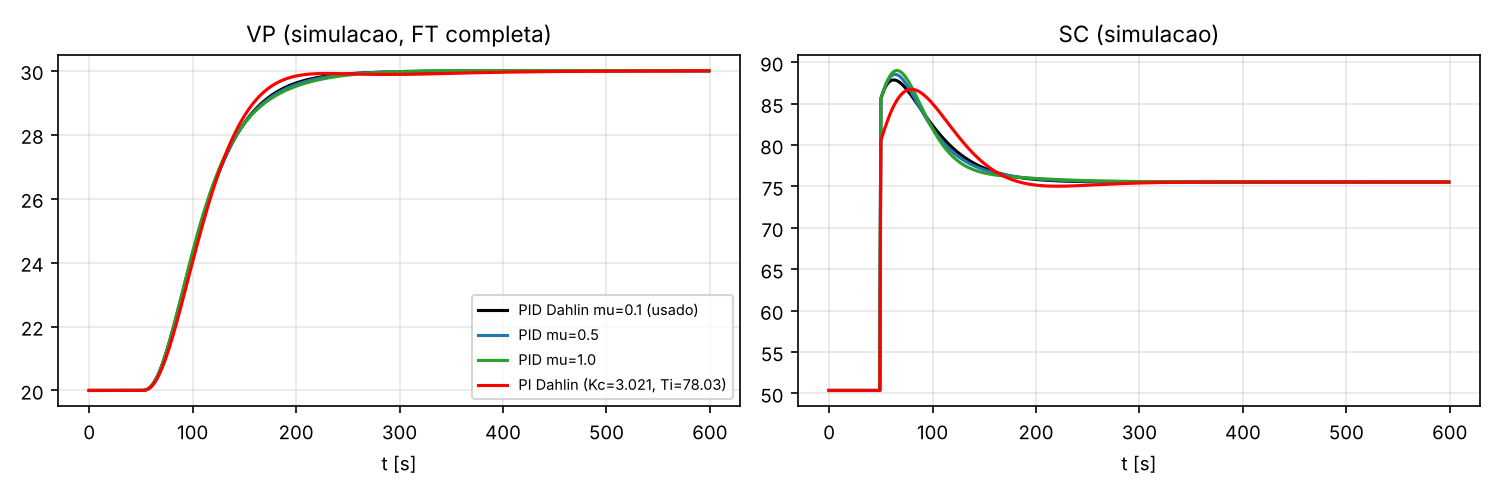
\includegraphics[width=.98\textwidth]{figs_exp/pi_x_pid.png}\caption{Simulação (FT completa): PID Dahlin ($\mu=0{,}1$, usado), PID com $\mu=0{,}5$ e $1{,}0$, e PI Dahlin. As quatro respostas praticamente coincidem.}\end{figure}
\begin{res}O PI de Dahlin dá praticamente a mesma VP ($t_{63}=71$ s contra 70 s; acomoda até mais rápido, 145 s contra 172 s), com $PM=70^\circ$ e $GM=9{,}5$ (folga confortável), e reduz o ganho de alta frequência de 38,8 para 3,0, isto é, \textbf{o efeito de 1 LSB no SC cai de 3,8 para 0,3 ponto (pelo menos 10 vezes menos), sem filtro nenhum}.\end{res}
\textbf{Recomendação (para relatório e prova):}
\begin{enumerate}
\item \textbf{Manter o relatório do item 1.1 como PID} (é o que o enunciado pede: ``sintonia de PID segundo a Tabela 7-4.1'') e \emph{documentar} o ruído com esta análise (causa, evidência e solução).
\item \textbf{Alternativa validada: PI de Dahlin} ($K_p=3{,}02$; $T_i=78{,}03$ s; $K_d=0$). É a resposta à pergunta ``precisa mudar para PI?'': não é obrigatório, mas \emph{funciona} e remove o ruído. Se for repetir o ensaio, \textbf{rode também um registro com PI} e confronte VP e SC (o SC do PI deve ficar limpo: desvio-padrão do SO próximo de 1 ponto, como a mediana atual).
\item \textbf{Se quiser manter a derivada}: (a) aumente $\mu$ (0,5 a 1,0) \emph{somente se} o bloco realmente usar o filtro (verifique o código); (b) filtre a VP antes do PID (média de 8 leituras do ADC ou um passa-baixa digital com constante $\approx1$ s); (c) aumente o tempo de execução do bloco PID (por exemplo 0,5 s: o pico por LSB cai para $39{,}15\cdot0{,}0976/0{,}5=7{,}6$ pontos); (d) filtro RC analógico na entrada do ADC.
\end{enumerate}
\begin{just}\textbf{Como confirmar o diagnóstico rapidamente na bancada:} repita o item 1.1 com $K_d=0$ (PI). Se a causa é a derivada, o SO deixa de ter picos (SO bruto $\approx$ mediana). Se ainda tiver picos, a causa está em outro ponto (por exemplo, o termo P e o ruído muito alto do ADC); nesse caso meça o ruído do ADC com a saída fixa.\end{just}

%------------------------------------------------------------------
\section{Item 1.2 experimental (Q12): transferência manual$\to$automático sem VP-tracking}
\subsection{Objetivo (seção 5-3.3 do livro)}
O \emph{bumpless VP-tracking} faz o SP acompanhar a VP enquanto o controlador está em manual. Assim, quando se passa para automático, $e=SP-VP=0$ e o SC não sofre salto. Sem o tracking, se o SP estiver diferente da VP no instante da transferência, o termo proporcional produz um salto $\Delta SC=K_p\,(SP-VP)$ (``bump'') e a VP é puxada bruscamente.
\subsection{O que foi feito}
\begin{enumerate}
\item Manual: $SO=10{,}37\to20{,}0\,\%$ e a VP sobe até $7{,}71\,\%$. Nesse período o \textbf{SP ficou em 0\,\%} (não acompanhou a VP: tracking desligado; compare com a Q11, em que o SP seguia a VP).
\item Em $t=577$ s o operador ajusta $SP=16{,}0\,\%$ (com a VP em $7{,}71$, isto é, $SP-VP=8{,}29$).
\item Em $t=593$ s passa para automático (SO manual $=20{,}0\,\%$).
\end{enumerate}
\subsection{Resultado}
\textbf{Previsto:} $\Delta SC=K_p(SP-VP)=3{,}523\cdot(16{,}00-7{,}71)=29{,}2$ pontos, isto é, $SC\approx20{,}0+29{,}2=49{,}2\,\%$ logo após a transferência.\\
\textbf{Medido:} $SO(593\text{--}600)=\{20{,}0;\ 30{,}1;\ 10{,}0;\ 49{,}7;\ 49{,}9;\ 99{,}9;\ 50{,}4;\ 31{,}5\}$ e \textbf{mediana de 595 a 615 s $=50{,}2\,\%$}: o SO saltou de $20$ para $\approx50\,\%$ (+$30$ pontos), exatamente o salto previsto (a diferença de 1 ponto é o termo integral e o ruído). Os valores 10, 30 e 99,9 são os picos da derivada da Seção~\ref{expruido}.
\begin{figure}[H]\centering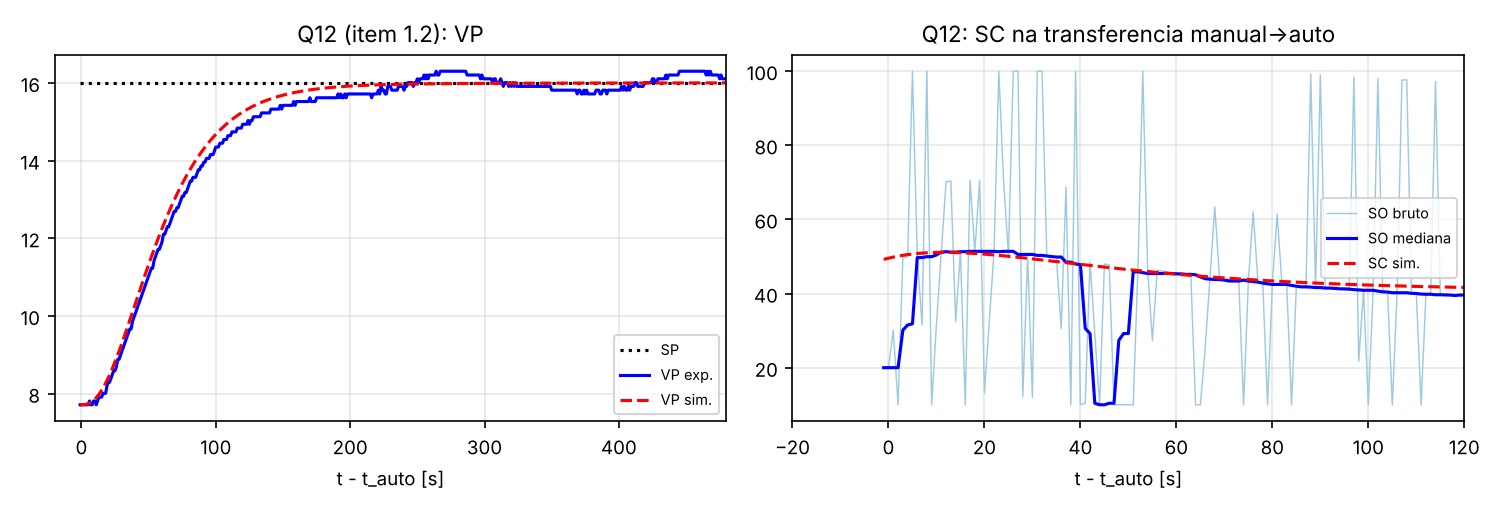
\includegraphics[width=.98\textwidth]{figs_exp/q12.png}\caption{Q12 (item 1.2). Esquerda: VP experimental e simulada após a transferência. Direita: SO na transferência (salto de $\sim30$ pontos em $t=0$) e SC simulado.}\end{figure}
A VP, que estava parada em $7{,}71\,\%$, sobe imediatamente em direção a 16\,\% como se o operador tivesse dado um degrau grande de SP, sem que o SC tenha sido ``pedido'': é o \emph{problema} que o tracking evita. A simulação (com a mesma sintonia, $SP=16$, $VP_0=7{,}71$, $SC_0=20$) reproduz a VP com RMS de $0{,}24\,\%$ e erro máximo de $0{,}45\,\%$ (VP máxima: 16,30 medida, 16,00 simulada).
\subsection{Comparação com o caso com VP-tracking (Q11)}
Na Q11, a transferência foi feita com $SP=VP=19{,}52$: o SO ficou em $\approx50\,\%$ (mediana $49{,}6\,\%$), sem salto (as oscilações isoladas são os picos de ruído). Resumo:
\begin{center}\small\begin{tabular}{lcc}\toprule & Sem tracking (Q12) & Com tracking (Q11)\\\midrule
$SP-VP$ na transferência & $+8{,}29$ & $0{,}00$\\ Salto previsto $K_p(SP-VP)$ & $+29{,}2$ & $0$\\ Salto medido (mediana do SO) & $+30$ (20$\to$50,2) & $\approx0$ (50,0$\to$49,6)\\\bottomrule\end{tabular}\end{center}
\begin{res}O experimento reproduz o problema: sem VP-tracking, a transferência manual$\to$automático com $SP\neq VP$ produz um salto de SC igual a $K_p(SP-VP)$ ($+30$ pontos medido, $+29{,}2$ previsto). Com tracking (Q11), não há salto.\end{res}

%------------------------------------------------------------------
\section{Item 1.3 experimental (Q13a e Q13b): anti reset windup}
\subsection{Fundamentos}
\textbf{O que é o windup.} A ação integral soma o erro no tempo, $I=K_i\!\int e\,dt$. Quando o atuador satura (SC no limite), o erro não consegue ser zerado, e a integral \emph{continua crescendo}, ``carregando'' um valor muito maior do que o atuador pode usar. Quando o SP volta a um valor alcançável, o erro muda de sinal, mas a integral só decresce à taxa $K_i|e|$ --- demora até que $u=K_pe+I$ saia da saturação. Durante esse tempo, a VP fica fora do controle.

\textbf{Anti reset windup} (seção 5-3.4): interromper a integração (ou descontar o excesso) enquanto o SC está saturado, de modo que $I$ fique perto do valor necessário no momento em que o SP deixa de ser inalcançável. A implementação por \emph{clamping} usada na simulação: $I[k+1]=I[k]+K_ie\Delta t$ \emph{exceto} se $u>u_{max}$ e $e>0$ ou $u<u_{min}$ e $e<0$.

\subsection{Alcance máximo e como o experimento foi planejado}
Com SC máximo de $99{,}94\,\%$: $VP_{max}=0{,}3963\cdot99{,}94-0{,}262=39{,}4\,\%$ (medido: $39{,}33$--$39{,}39\,\%$ em Q13a). Logo, $SP=55\,\%$ é \emph{inalcançável} por uma larga margem e o SC fica saturado em 99,94\,\% durante todo o tempo em que o SP está em 55\,\%.

\subsection{Linha do tempo extraída dos dados}
\begin{center}\small
\begin{tabular}{lcc}\toprule Evento & Q13a (sem AW) & Q13b (com AW)\\\midrule
Malha fechada (SO manual 20\,\%) & $t=820$ s ($VP=7{,}5$) & $t=38$ s ($VP=6{,}05$)\\
SP $\to55\,\%$ & $t=822$ s & $t=43$ s\\
Tempo com SP inalcançável & 449 s & 501 s\\
VP máxima no patamar & 39,33\,\% & 38,16\,\%\\
SP $\to20\,\%$ & $t=1271$ s & $t=544$ s\\\bottomrule\end{tabular}\end{center}
\begin{figure}[H]\centering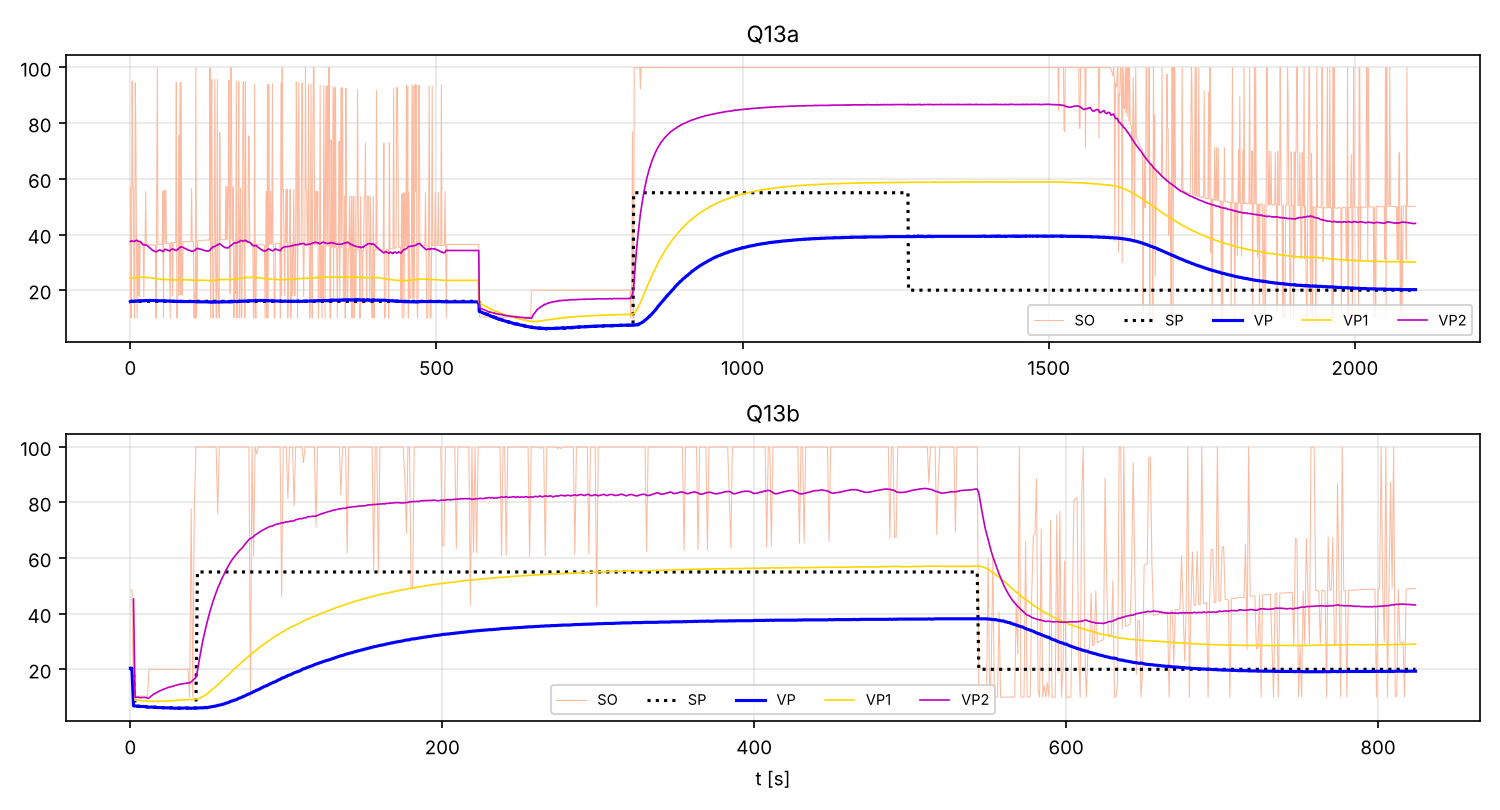
\includegraphics[width=.98\textwidth]{figs_exp/q13_completo.png}\caption{Registros completos de Q13a (acima) e Q13b (abaixo): SO, SP, VP, VP1 e VP2.}\end{figure}
\subsection{Resultado: o que acontece depois que o SP volta a 20\,\%}
\begin{figure}[H]\centering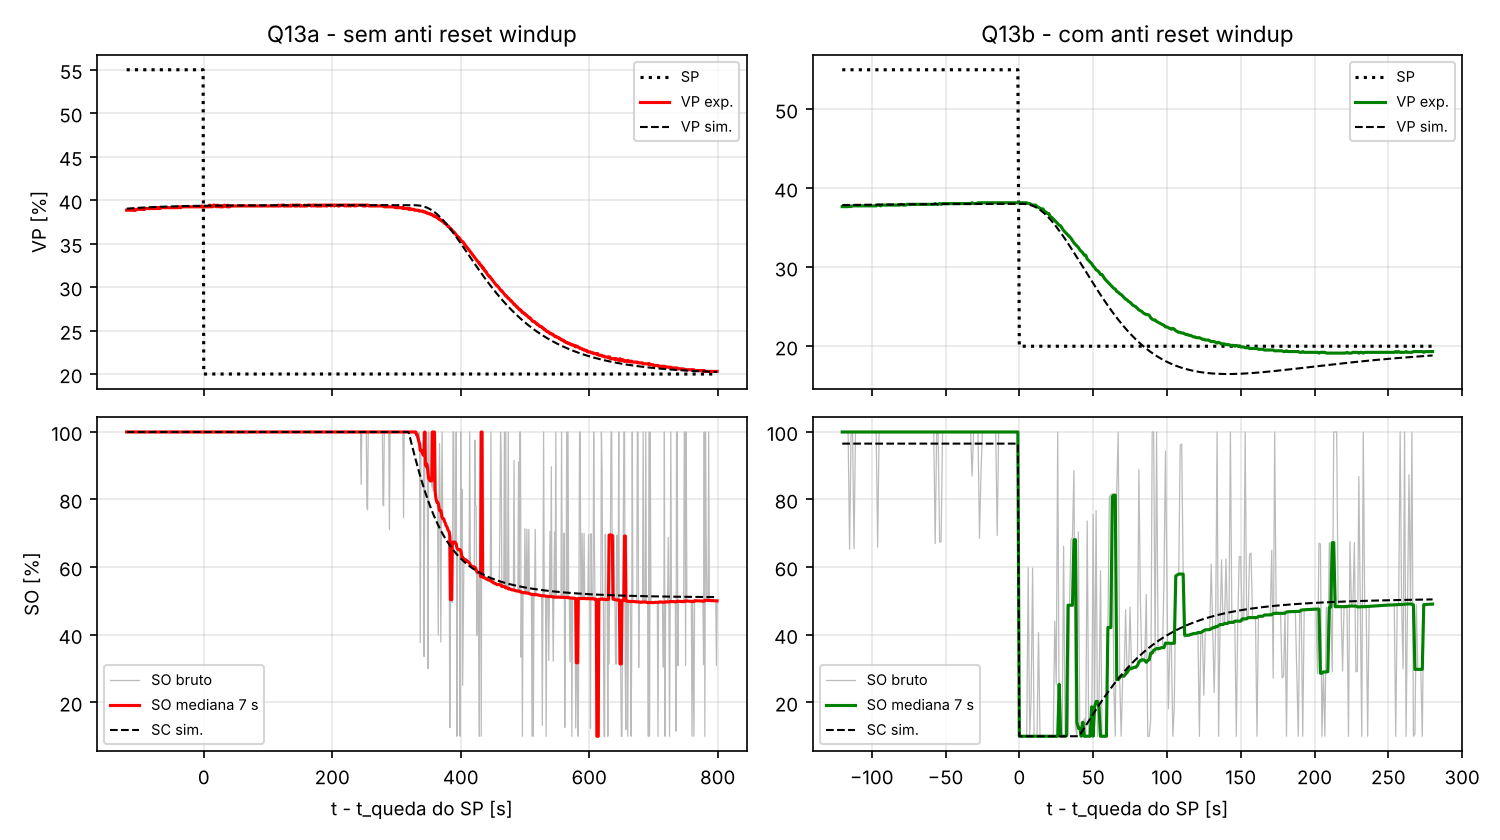
\includegraphics[width=.98\textwidth]{figs_exp/q13.png}\caption{Q13 alinhado no instante da queda do SP (t=0). Esquerda: sem anti-windup. Direita: com anti-windup. Linhas tracejadas: simulação.}\end{figure}
\begin{center}\small
\resizebox{\textwidth}{!}{\begin{tabular}{lcc}\toprule Medida (a partir da queda do SP) & Q13a: sem AW & Q13b: com AW\\\midrule
O SO sai da saturação (mediana $<95\,\%$) & \textbf{337 s} depois & \textbf{0 s} (imediato)\\
A VP começa a cair (0,5 ponto abaixo do máximo) & \textbf{342 s} depois & \textbf{13 s} depois\\
A VP fica dentro de $\pm1$ ponto de 20\,\% & 700 s & 123 s\\\midrule
Simulação: SC sai da saturação & 326 s (sem AW) & 0 s (com AW)\\
Simulação: VP cai 0,5 ponto & 355 s (sem AW) & 12 s (com AW)\\
Erro RMS VP experimental $\times$ simulado & \textbf{0,43\,\%} (sem AW) / 11,0\,\% (com AW) & \textbf{1,62\,\%} (com AW) / 9,2\,\% (sem AW)\\\bottomrule\end{tabular}}\end{center}
\textbf{Interpretação.}
\begin{itemize}
\item \textbf{Sem anti-windup (Q13a):} depois da queda do SP, o SO permanece em 99,94\,\% por \textbf{337 s} e a VP permanece em 39,3\,\% por $\approx340$ s, \emph{mesmo com o SP em 20\,\% e erro de $-19$ pontos}. O controlador está ``cego'': o integrador acumulou, durante os 449 s de saturação, um valor muito acima do que o atuador entrega. Só depois que o integrador desce é que $u=K_pe+I$ cai abaixo de 99,94 e a VP finalmente começa a descer. Só chega a $\pm1$ ponto de 20\,\% depois de $\approx700$ s.
\item \textbf{Com anti-windup (Q13b):} o SO deixa a saturação \emph{imediatamente} e a VP começa a cair 13 s depois (o atraso de 13 s é a dinâmica do circuito: $\Vc3$ é de 3ª ordem e só começa a cair depois que $\Vc1$ e $\Vc2$ caem), chegando a $\pm1$ ponto de 20\,\% em 123 s, \textbf{5,7 vezes mais rápido} que sem anti-windup (700 s).
\item \textbf{Quantificando o windup (conta feita com os dados):} durante os 449 s com SP$=55$ (erro positivo de 47 pontos no início e 16 no fim), a integral acumulou $I=20+K_i\sum e\,\Delta t=20+0{,}03872\cdot\sum(SP-VP)=414$ pontos de SC (em regime final, para $SP=20$, bastariam $I\approx(20+0{,}26)/0{,}3971=51$). Logo após a queda do SP, o erro vale $20-39{,}3=-19{,}3$ e o termo proporcional $K_pe=3{,}523\cdot(-19{,}3)=-68$; o controlador só sai da saturação quando $u=K_pe+I<99{,}94$, isto é, $I<168$. A integral precisa descer $414-168=246$ pontos à taxa $K_i|e|=0{,}03872\cdot19{,}3=0{,}75$ ponto/s:
\[t_{saida}\approx\frac{246}{0{,}75}=328\ \mathrm{s}\qquad(\text{medido: }337\ \mathrm{s}).\]
A estimativa independente da simulação (328 s) confere com o dado (337 s): o atraso é exatamente o tempo de ``desenrolar'' o integrador.
\item \textbf{A simulação reproduz cada caso com a estrutura certa:} o modelo \emph{sem} anti-windup reproduz a Q13a (RMS 0,43\,\%; SO sai da saturação em 326 s contra 337 s medidos); o modelo \emph{com} anti-windup (clamping) reproduz a Q13b (RMS 1,62\,\%, mesmo tempo de saída da saturação, VP caindo em 12 s contra 13 s). Trocando as estruturas, o erro explode (11,0\,\% e 9,2\,\%): a simulação \emph{discrimina} qual é qual, o que confirma que a Q13a é sem proteção e a Q13b com proteção.
\item \textbf{Diferenças residuais na Q13b} (RMS 1,6\,\%, concentrado depois da queda do SP): (i) o SC médio no patamar saturado foi 96,6\,\% e não 99,94\,\% (retificação do ruído da derivada); (ii) depois da queda, o SC deveria ficar em 10\,\%, mas o SO médio foi 25--35\,\% pelos picos, o que retarda a queda da VP (a VP experimental cai mais devagar que a simulada, sem o \emph{undershoot} de $\approx3$ pontos que a simulação com clamping prevê). Ambos os efeitos são consequência do mesmo ruído da Seção~\ref{expruido}.
\end{itemize}
\begin{res}O experimento reproduz o problema do windup: sem anti-windup, depois de 449 s com o SP inalcançável, a VP fica \textbf{340 s} presa no valor máximo ($39{,}3\,\%$) e só atinge $20\pm1\,\%$ em $\approx700$ s; com anti-windup o SC sai da saturação na hora, a VP reage em 13 s (dinâmica da planta) e chega a $20\pm1\,\%$ em 123 s.\end{res}

%------------------------------------------------------------------
\section{Conclusões dos experimentos da Questão 1}
\begin{enumerate}
\item \textbf{Modelo validado no dia do ensaio:} inclinação estática $0{,}3963$ (teórico $0{,}3971$), offset de $-0{,}26$ ponto e dinâmica reproduzida com RMS de 0,2--0,8\,\% quando a planta é excitada com o SO medido.
\item \textbf{Item 1.1:} a sintonia de Dahlin ($\tau_c=40$ s) funcionou: sem sobressinal significativo, erro nulo em regime, salto de SC igual a $K_p\Delta SP$. A resposta experimental é $\approx13\,\%$ mais lenta que a simulada ($t_{63}$ de 79 contra 70 s), coerente com a diferença de 4--6\,\% nas constantes de tempo já observada e com o ruído do SC.
\item \textbf{SO ``instável'':} é \textbf{ruído no sinal de controle}, não instabilidade da malha: a derivada amplifica os degraus de 1 LSB (0,098\,\%) do ADC (probabilidade de pico 8,7 vezes maior nas transições da VP); os picos, de dezenas de pontos, são cortados pelos limites $\approx10$ e $\approx99{,}94\,\%$ do SC. O filtro $\mu=0{,}1$ deveria limitar o pico a $\approx3{,}4$ pontos, mas os picos observados são $\sim10$ vezes maiores: o filtro não atua como projetado no bloco usado.
\item \textbf{PI:} não é obrigatório para a estabilidade, mas é a correção mais simples: o PI de Dahlin ($K_c=3{,}02$; $T_i=78{,}03$ s) dá VP praticamente idêntica ($t_{63}=71$ s, $PM=70^\circ$) com o ganho de alta frequência 13 vezes menor. Recomendo registrar um ensaio com PI para confirmar.
\item \textbf{Item 1.2:} sem VP-tracking, o SC saltou $+30$ pontos na transferência (previsto $K_p(SP-VP)=29{,}2$); com tracking (Q11), não há salto.
\item \textbf{Item 1.3:} sem anti-windup a VP fica presa em $39{,}3\,\%$ por $\approx340$ s depois da queda do SP, e só chega a $20\pm1\,\%$ em 700 s; com anti-windup, em 123 s. A simulação com a estrutura correta reproduz cada ensaio com RMS $\le1{,}6\,\%$.
\end{enumerate}
\textbf{Limitações:} (i) a sintonia usada (Dahlin) foi inferida do salto do SO, não de anotação; (ii) os picos de SO são amostrados a 1 s e portanto subestimados; (iii) o código do bloco PID não foi analisado, o que impede afirmar a causa exata do filtro derivativo ineficaz; (iv) só há um ensaio de cada tipo, sem repetição.
